\documentclass[11pt]{article}
\usepackage[a4paper,margin=1in]{geometry}
\usepackage{amsmath,amssymb,amsthm,mathtools}
\usepackage{booktabs}
\usepackage{enumitem}
\usepackage{graphicx}
\usepackage{microtype}
\usepackage{hyperref}
\usepackage[nameinlink,capitalise]{cleveref}
\usepackage[numbers,sort&compress]{natbib}

\newtheorem{theorem}{Theorem}[section]
\newtheorem{proposition}[theorem]{Proposition}
\newtheorem{corollary}[theorem]{Corollary}
\theoremstyle{definition}
\newtheorem{definition}[theorem]{Definition}
\theoremstyle{remark}
\newtheorem{remark}[theorem]{Remark}
\newcommand{\norm}[1]{\left\lVert#1\right\rVert}
\newcommand{\tr}{\operatorname{tr}}
\newcommand{\E}{\mathcal E}

\title{Projector-Lipschitz Propagation Envelopes\\
\large Why Universal Unit Tail Propagation Is False}
\author{Liang Wang}
\date{July 2026}

\begin{document}
\maketitle

\begin{abstract}
The exact hybrid budgets of RH-97 show no tail amplification on the archived
packet chains: every propagated quotient contribution is no larger than its
local loss.  We test whether this unit behavior can be promoted to a theorem.
It cannot.

We first derive the correct conditional factorization.  For rank-$r$ packets
$U,V$ and endpoint Gramian $G$,
\[
 |\E_G(U)-\E_G(V)|
 \le\norm G_F\norm{UU^*-VV^*}_F.
\]
If an adaptive rank-$r$ Ritz packet has capture loss $\varepsilon$ relative
to the leading rank-$r$ packet of a compressed Hermitian matrix with gap
$\gamma=\lambda_r-\lambda_{r+1}>0$, then
\[
 \norm{P_{\rm ad}-P_{\rm full}}_F
 \le\sqrt{\frac{2\varepsilon}{\gamma}}.
\]
If the future full block is projector-Lipschitz with constant $L$, these give
the conditional projector block envelope
\[
 |\Delta_{\rm end}|
 \le\norm{G_N}_F L\sqrt{\frac{2\varepsilon}{\gamma}}.
\]

All 38 production omissions generated by the three RH-96 cutoffs satisfy the
gap-to-projector, endpoint Lipschitz, and combined conditional bounds.  Tail
amplification is at most $1+4\times10^{-16}$ numerically.  Projector secant
amplification nevertheless reaches $8.85112$, showing that endpoint energy is
less sensitive than packet geometry.

We then give an explicit $6\times6$, trace-one, strictly positive two-step
projected-cross Ritz counterexample.  A width-one first update has validated
local loss at most $5.28909\times10^{-4}$ relative to width two.  After one
common width-two future refresh, the endpoint tail difference is at least
$2.35338\times10^{-2}$, a certified amplification greater than $44.4949$.
Thus unit propagation is false even for normalized positive Gramians.

The missing route object is not a universal constant one, but a
neighborhood-uniform projector-Lipschitz bound for the actual separated
reduced maps.  No such uniform bound, repeated-block theorem, Hilbert--Polya
operator, zero identification, or Riemann Hypothesis result is claimed.
\end{abstract}

\noindent\textbf{Keywords:} spectral projector; Lipschitz propagation; Ritz
gap; Grassmann distance; counterexample; validated numerics.

\medskip
\noindent\textbf{MSC 2020:} 47A75; 15A18; 65F15; 65G20; 37C30.

\section{Introduction}

RH-97 decomposes the endpoint effect of adaptive weak-mode omissions into
exact nonlinear hybrid contributions \citep{WangHybrid2026}.  On all archived
chains, the absolute endpoint contribution of each omission is no larger than
its local one-step tail loss, up to roundoff.  If this were a structural
nonexpansiveness theorem, the replay-free horizon budget would be immediate.

There is reason for caution.  A projected-cross Ritz update is not a metric
projection in one fixed Hilbert geometry.  Its trial space depends on the
incoming packet, the Gramian changes with time, and a small local energy
difference can correspond to a packet displacement that a later Gramian sees
strongly.  Ritz monotonicity controls one packet under one Gramian; it does not
compare two packet histories.

The paper therefore separates three transformations:
\[
\begin{aligned}
 \text{local energy loss}
 &\longrightarrow \text{local projector displacement}\\
 &\longrightarrow \text{future projector displacement}
 \longrightarrow \text{endpoint energy effect}.
\end{aligned}
\]
The first arrow is controlled by a compressed spectral gap.  The last is
controlled by the endpoint Gram norm.  The middle arrow is the genuinely
dynamical object: a projector-Lipschitz constant for the future full block.

This factorization gives a valid conditional theorem.  More importantly, a
small explicit counterexample proves that the middle factor cannot be
silently replaced by one.  The production data remain favorable, but their
favorable behavior must be proved from the specific map family.

\section{Endpoint tail/projector Lipschitz theorem}
\label{sec:endpoint}

For an isometric rank-$r$ packet $V$, let $P_V=VV^*$ and
\[
 \E_G(V)=\tr G-\tr(GP_V).
\]

\begin{theorem}[Endpoint tail/projector Lipschitz theorem]
\label{thm:endpoint}
For $G=G^*$ and any two rank-$r$ packets $U,V$,
\begin{equation}
 |\E_G(U)-\E_G(V)|
 \le\norm G_F\norm{P_U-P_V}_F.
 \label{eq:endpoint}
\end{equation}
\end{theorem}

\begin{proof}
The trace terms cancel:
\[
 \E_G(U)-\E_G(V)=\tr\bigl(G(P_V-P_U)\bigr).
\]
Apply the Frobenius Cauchy--Schwarz inequality.
\end{proof}

The theorem is exact and global.  It does not require a spectral gap or a
common trial space.  Its usefulness depends on controlling the future packet
projector distance.

\section{Local gap loss-to-projector theorem}
\label{sec:local}

Let $H=H^*$ be a compressed Ritz matrix of dimension at least $r+1$, with
eigenvalues
\[
 \lambda_1\ge\cdots\ge\lambda_r>
 \lambda_{r+1}\ge\cdots.
\]
Let $P_*$ be its leading rank-$r$ spectral projector and $Q$ any rank-$r$
orthogonal projector in the same compressed space.  Define the capture loss
\[
 \varepsilon=\tr(HP_*)-\tr(HQ)\ge0.
\]

\begin{theorem}[Local gap loss-to-projector theorem]
\label{thm:local}
With $\gamma=\lambda_r-\lambda_{r+1}>0$,
\begin{equation}
 \norm{P_*-Q}_F
 \le\sqrt{\frac{2\varepsilon}{\gamma}}.
 \label{eq:local}
\end{equation}
\end{theorem}

\begin{proof}
Work in an eigenbasis of $H$.  If $q_i$ are the diagonal entries of $Q$ in
that basis, then $0\le q_i\le1$ and $\sum_iq_i=r$.  Hence
\begin{align*}
 \varepsilon
 &=\sum_{i\le r}\lambda_i(1-q_i)
   -\sum_{i>r}\lambda_iq_i\\
 &\ge\gamma\sum_{i>r}q_i
 =\gamma\bigl(r-\tr(P_*Q)\bigr).
\end{align*}
For rank-$r$ projectors,
\[
 \norm{P_*-Q}_F^2=2r-2\tr(P_*Q),
\]
which gives \eqref{eq:local}.  This is the elementary sin-theta energy bound
behind standard spectral projector perturbation estimates
\citep{DavisKahan1970,StewartSun1990}.
\end{proof}

In the adaptive enrichment setting, $Q$ is the adaptive packet embedded in
the full-width compressed basis, and $P_*$ is the full-width leading packet.
The local quotient loss is exactly $\varepsilon$.

\section{Conditional projector block envelope}
\label{sec:conditional}

Let $\mathcal F_{j+1:N}$ denote the future composition of full-width packet
refresh maps from time $j+1$ to $N$.  Suppose that on a set containing two
local outputs,
\begin{equation}
 \norm{P_{\mathcal F_{j+1:N}(U)}
            -P_{\mathcal F_{j+1:N}(V)}}_F
 \le L_{j,N}\norm{P_U-P_V}_F.
 \label{eq:block-lipschitz}
\end{equation}

\begin{corollary}[Conditional projector block envelope]
\label{cor:conditional}
If the local full-width compressed gap is $\gamma_j>0$ and the local
adaptive capture loss is $\varepsilon_j$, then
\begin{equation}
 |\Delta_{j,N}|
 \le\norm{G_N}_F L_{j,N}
 \sqrt{\frac{2\varepsilon_j}{\gamma_j}}.
 \label{eq:conditional}
\end{equation}
\end{corollary}

\begin{proof}
Apply \cref{thm:local} at time $j$, then
\eqref{eq:block-lipschitz}, and finally \cref{thm:endpoint}.
\end{proof}

The bound identifies the missing constant precisely.  A pairwise secant
value
\[
 L_{j,N}^{\rm sec}
 =\frac{\norm{P_{\mathcal F(U)}-P_{\mathcal F(V)}}_F}
 {\norm{P_U-P_V}_F}
\]
certifies one concrete pair a posteriori.  A replay-free theorem needs a
uniform $L_{j,N}$ on a neighborhood containing all admissible quotient
outputs.

\section{Universal unit propagation is false}
\label{sec:counterexample}

We now reject the tempting assertion
\[
 |\Delta_{j,N}|\le\varepsilon_j
\]
for arbitrary normalized positive Gram sequences.

\begin{proposition}[Strictly positive two-step counterexample]
\label{prop:counterexample}
There exist $6\times6$ real symmetric positive definite matrices
$G_1,G_2$ with $\tr G_1=\tr G_2=1$, and a rank-two initial packet $V$, such
that:
\begin{enumerate}[leftmargin=2em]
\item at time one, width one has positive tail loss $\varepsilon$ relative to
width two;
\item applying the same width-two refresh under $G_2$ to both outputs gives
endpoint tail difference $\Delta$ satisfying
\[
 \frac{|\Delta|}{\varepsilon}>44.4949.
\]
\end{enumerate}
\end{proposition}

\begin{proof}
The matrices and packet are archived as exact binary inputs in the audit
record.  Their smallest binary64 eigenvalue lower diagnostics are
$5.55\times10^{-3}$ and $1.44\times10^{-7}$, respectively, and both traces
are exactly one in binary64.

At 384-bit Arb precision, the local loss has outward upper bound
\[
 \varepsilon\le5.2890877381\times10^{-4},
\]
while the absolute endpoint effect has outward lower bound
\[
 |\Delta|\ge2.3533757224\times10^{-2}.
\]
Division of the outward bounds gives
$|\Delta|/\varepsilon>44.49492689$.  The endpoint
tail/projector Lipschitz bound remains green, so the amplification is genuine
and not a failed numerical inequality.
\end{proof}

\begin{remark}
The counterexample is not a claim about the production Gaussian family.  It
shows that positivity, trace normalization, and projected-cross Ritz
structure alone do not imply unit propagation.
\end{remark}

\section{Production audit}
\label{sec:audit}

We replay all omissions generated by the thresholds
$10^{-8},10^{-6},10^{-4}$ on the ten RH-96 channels, giving 38 local/future
pairs.  For each pair we record:
\begin{enumerate}[leftmargin=2em]
\item the local adaptive/full capture loss and full compressed gap;
\item the actual local projector distance and the bound
\eqref{eq:local};
\item the future full-block endpoint projector distance and secant multiplier;
\item the endpoint tail effect and bound \eqref{eq:endpoint};
\item the combined conditional bound \eqref{eq:conditional}, using the
pairwise secant.
\end{enumerate}
Quadratic tail forms are evaluated from exact binary packets in Arb at 384
bits \citep{Rump2010}.

All 38 local gap-distance bounds close.  All 38 endpoint
tail/projector bounds close.  All 38 conditional secant envelopes close.
The largest gap-distance slack factor is $19.29$.

Tail amplification is numerically at most
\[
 1.0000000000000004,
\]
so all 38 pairs are unit-propagating within a $10^{-12}$ roundoff allowance.
The strict outward comparison is inconclusive at fourteen near-equality
cases, mostly omissions at the endpoint itself.

Packet geometry behaves differently.  The largest projector secant
multiplier is
\[
 8.85111975
\]
for the primary threshold, and the $10^{-6}$ family reaches $7.75018$.
Future refresh can amplify Grassmann displacement even while the endpoint
tail functional suppresses its energetic effect.

\begin{figure}[t]
\centering
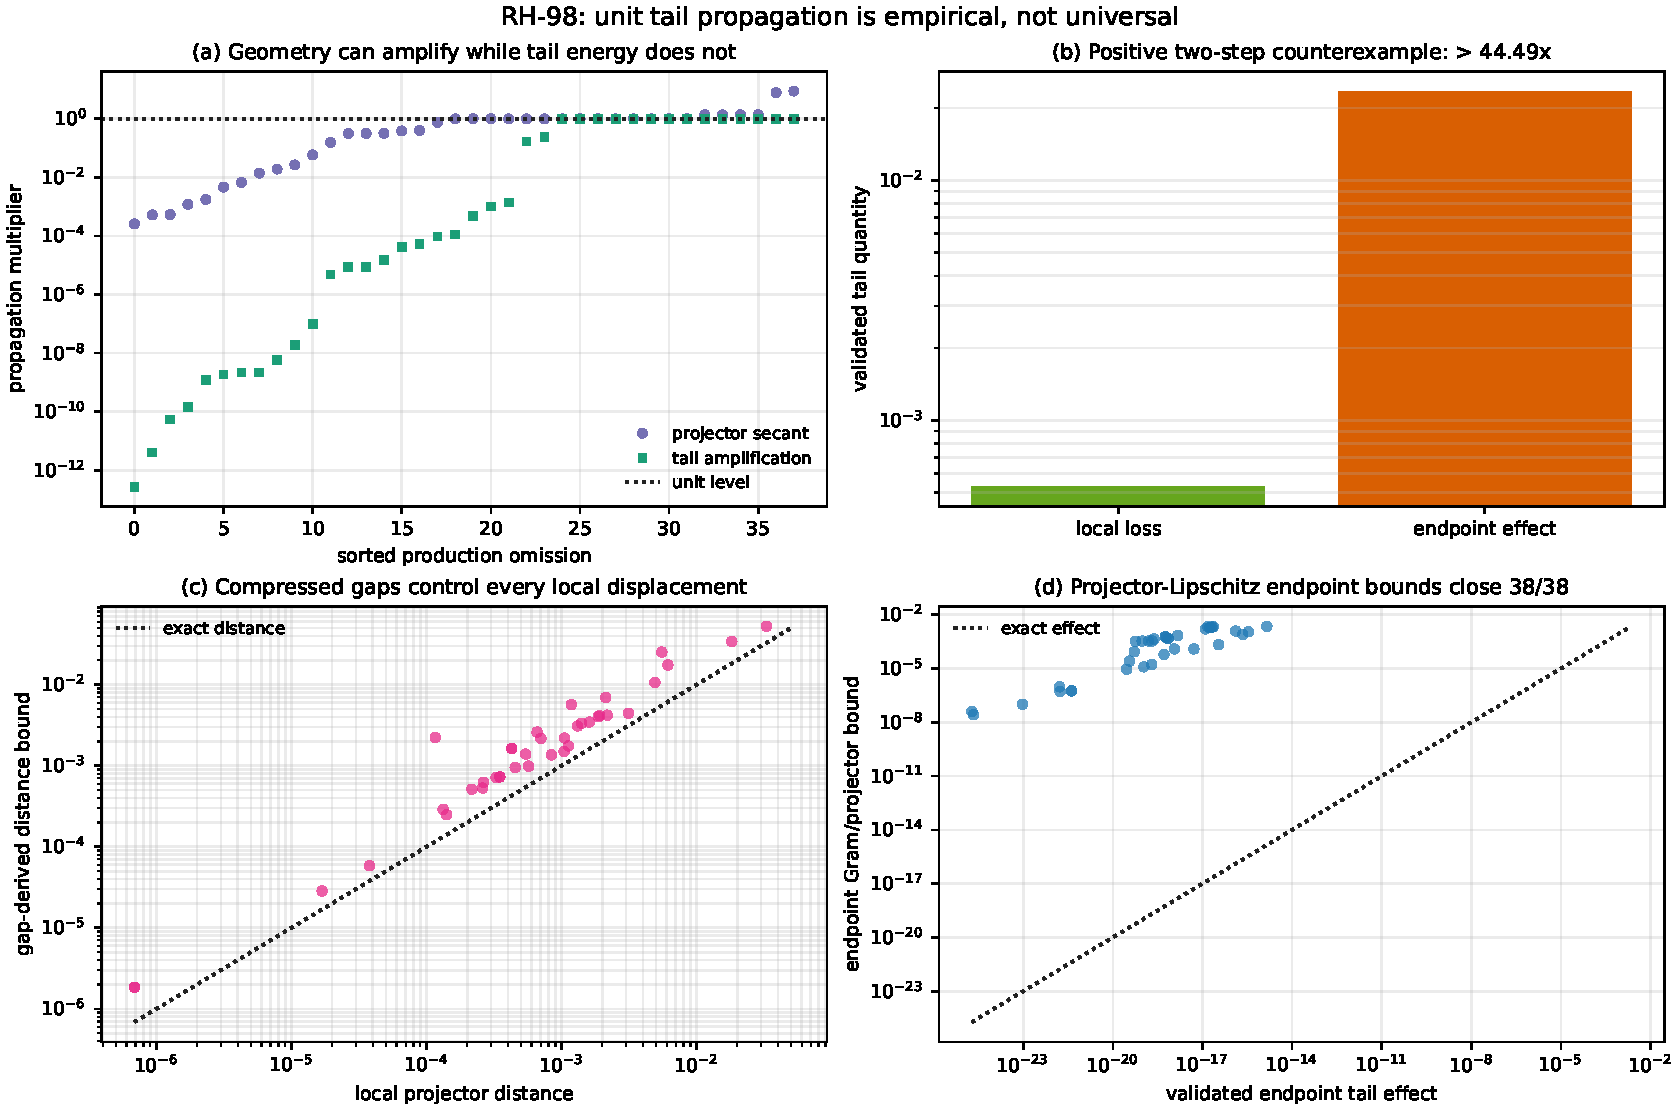
\includegraphics[width=\textwidth]{figures/projector_lipschitz_propagation_barrier.pdf}
\caption{Production pairs satisfy the conditional projector envelope, but
projector secants can exceed eight.  The explicit positive counterexample
rejects universal unit tail propagation by a factor greater than forty-four.}
\label{fig:audit}
\end{figure}

\section{Next gate: a differential projector tube}

The correct RH-99 target is a neighborhood-uniform version of
\eqref{eq:block-lipschitz}.  For a separated spectral projector, its
Fr\'echet derivative is represented by a reduced resolvent or Sylvester
equation.  One should differentiate the complete projected-cross Ritz map,
including:
\begin{itemize}[leftmargin=2em]
\item the incoming packet projector;
\item the projected cross operator and selected singular subspace;
\item the enriched compressed matrix;
\item the leading compressed Ritz projector.
\end{itemize}
If each selected singular and Ritz cluster remains separated on a verified
projector ball, derivative norms can be integrated to obtain a genuine local
Lipschitz constant.  Branch changes or gap collapse would instead provide a
precise negative result.

\section{Claim boundary}

The endpoint tail/projector Lipschitz theorem, local gap loss-to-projector
theorem, conditional projector block envelope, and positive-definite
counterexample are exact finite-dimensional results.  The production secants
are pairwise a posteriori diagnostics.  We do not prove a neighborhood-uniform
refresh Lipschitz constant, a replay-free uniform block envelope,
repeated-block contraction, Stage-A closure, a Hilbert--Polya operator,
zeta-zero identification, or the Riemann Hypothesis.

\section{Conclusion}

Unit propagation is false.  The archived family happens to show unit tail
behavior, but a normalized positive two-step Ritz system can amplify local
loss by more than forty-four.  The valid route is projector-metric:
compressed gaps convert loss to displacement, future map Lipschitz constants
propagate displacement, and the endpoint Gram converts it back to energy.

All production pairs satisfy this factorized envelope.  The next paper must
turn their secant constants into verified differential tubes.

\bibliographystyle{plainnat}
\bibliography{references}

\end{document}
